% Options for packages loaded elsewhere
\PassOptionsToPackage{unicode}{hyperref}
\PassOptionsToPackage{hyphens}{url}
%
\documentclass[
]{article}
\usepackage{lmodern}
\usepackage{amssymb,amsmath}
\usepackage{ifxetex,ifluatex}
\ifnum 0\ifxetex 1\fi\ifluatex 1\fi=0 % if pdftex
  \usepackage[T1]{fontenc}
  \usepackage[utf8]{inputenc}
  \usepackage{textcomp} % provide euro and other symbols
\else % if luatex or xetex
  \usepackage{unicode-math}
  \defaultfontfeatures{Scale=MatchLowercase}
  \defaultfontfeatures[\rmfamily]{Ligatures=TeX,Scale=1}
\fi
% Use upquote if available, for straight quotes in verbatim environments
\IfFileExists{upquote.sty}{\usepackage{upquote}}{}
\IfFileExists{microtype.sty}{% use microtype if available
  \usepackage[]{microtype}
  \UseMicrotypeSet[protrusion]{basicmath} % disable protrusion for tt fonts
}{}
\makeatletter
\@ifundefined{KOMAClassName}{% if non-KOMA class
  \IfFileExists{parskip.sty}{%
    \usepackage{parskip}
  }{% else
    \setlength{\parindent}{0pt}
    \setlength{\parskip}{6pt plus 2pt minus 1pt}}
}{% if KOMA class
  \KOMAoptions{parskip=half}}
\makeatother
\usepackage{xcolor}
\IfFileExists{xurl.sty}{\usepackage{xurl}}{} % add URL line breaks if available
\IfFileExists{bookmark.sty}{\usepackage{bookmark}}{\usepackage{hyperref}}
\hypersetup{
  pdftitle={STAT 33B Homework 3},
  pdfauthor={Ming Fong (3035619833)},
  hidelinks,
  pdfcreator={LaTeX via pandoc}}
\urlstyle{same} % disable monospaced font for URLs
\usepackage[margin=1in]{geometry}
\usepackage{color}
\usepackage{fancyvrb}
\newcommand{\VerbBar}{|}
\newcommand{\VERB}{\Verb[commandchars=\\\{\}]}
\DefineVerbatimEnvironment{Highlighting}{Verbatim}{commandchars=\\\{\}}
% Add ',fontsize=\small' for more characters per line
\usepackage{framed}
\definecolor{shadecolor}{RGB}{248,248,248}
\newenvironment{Shaded}{\begin{snugshade}}{\end{snugshade}}
\newcommand{\AlertTok}[1]{\textcolor[rgb]{0.94,0.16,0.16}{#1}}
\newcommand{\AnnotationTok}[1]{\textcolor[rgb]{0.56,0.35,0.01}{\textbf{\textit{#1}}}}
\newcommand{\AttributeTok}[1]{\textcolor[rgb]{0.77,0.63,0.00}{#1}}
\newcommand{\BaseNTok}[1]{\textcolor[rgb]{0.00,0.00,0.81}{#1}}
\newcommand{\BuiltInTok}[1]{#1}
\newcommand{\CharTok}[1]{\textcolor[rgb]{0.31,0.60,0.02}{#1}}
\newcommand{\CommentTok}[1]{\textcolor[rgb]{0.56,0.35,0.01}{\textit{#1}}}
\newcommand{\CommentVarTok}[1]{\textcolor[rgb]{0.56,0.35,0.01}{\textbf{\textit{#1}}}}
\newcommand{\ConstantTok}[1]{\textcolor[rgb]{0.00,0.00,0.00}{#1}}
\newcommand{\ControlFlowTok}[1]{\textcolor[rgb]{0.13,0.29,0.53}{\textbf{#1}}}
\newcommand{\DataTypeTok}[1]{\textcolor[rgb]{0.13,0.29,0.53}{#1}}
\newcommand{\DecValTok}[1]{\textcolor[rgb]{0.00,0.00,0.81}{#1}}
\newcommand{\DocumentationTok}[1]{\textcolor[rgb]{0.56,0.35,0.01}{\textbf{\textit{#1}}}}
\newcommand{\ErrorTok}[1]{\textcolor[rgb]{0.64,0.00,0.00}{\textbf{#1}}}
\newcommand{\ExtensionTok}[1]{#1}
\newcommand{\FloatTok}[1]{\textcolor[rgb]{0.00,0.00,0.81}{#1}}
\newcommand{\FunctionTok}[1]{\textcolor[rgb]{0.00,0.00,0.00}{#1}}
\newcommand{\ImportTok}[1]{#1}
\newcommand{\InformationTok}[1]{\textcolor[rgb]{0.56,0.35,0.01}{\textbf{\textit{#1}}}}
\newcommand{\KeywordTok}[1]{\textcolor[rgb]{0.13,0.29,0.53}{\textbf{#1}}}
\newcommand{\NormalTok}[1]{#1}
\newcommand{\OperatorTok}[1]{\textcolor[rgb]{0.81,0.36,0.00}{\textbf{#1}}}
\newcommand{\OtherTok}[1]{\textcolor[rgb]{0.56,0.35,0.01}{#1}}
\newcommand{\PreprocessorTok}[1]{\textcolor[rgb]{0.56,0.35,0.01}{\textit{#1}}}
\newcommand{\RegionMarkerTok}[1]{#1}
\newcommand{\SpecialCharTok}[1]{\textcolor[rgb]{0.00,0.00,0.00}{#1}}
\newcommand{\SpecialStringTok}[1]{\textcolor[rgb]{0.31,0.60,0.02}{#1}}
\newcommand{\StringTok}[1]{\textcolor[rgb]{0.31,0.60,0.02}{#1}}
\newcommand{\VariableTok}[1]{\textcolor[rgb]{0.00,0.00,0.00}{#1}}
\newcommand{\VerbatimStringTok}[1]{\textcolor[rgb]{0.31,0.60,0.02}{#1}}
\newcommand{\WarningTok}[1]{\textcolor[rgb]{0.56,0.35,0.01}{\textbf{\textit{#1}}}}
\usepackage{graphicx}
\makeatletter
\def\maxwidth{\ifdim\Gin@nat@width>\linewidth\linewidth\else\Gin@nat@width\fi}
\def\maxheight{\ifdim\Gin@nat@height>\textheight\textheight\else\Gin@nat@height\fi}
\makeatother
% Scale images if necessary, so that they will not overflow the page
% margins by default, and it is still possible to overwrite the defaults
% using explicit options in \includegraphics[width, height, ...]{}
\setkeys{Gin}{width=\maxwidth,height=\maxheight,keepaspectratio}
% Set default figure placement to htbp
\makeatletter
\def\fps@figure{htbp}
\makeatother
\setlength{\emergencystretch}{3em} % prevent overfull lines
\providecommand{\tightlist}{%
  \setlength{\itemsep}{0pt}\setlength{\parskip}{0pt}}
\setcounter{secnumdepth}{-\maxdimen} % remove section numbering
\ifluatex
  \usepackage{selnolig}  % disable illegal ligatures
\fi

\title{STAT 33B Homework 3}
\author{Ming Fong (3035619833)}
\date{Oct 8, 2020}

\begin{document}
\maketitle

This homework is due \textbf{Oct 8, 2020} by 11:59pm PT.

Homeworks are graded for correctness.

As you work, write your answers in this notebook. Answer questions with
complete sentences, and put code in code chunks. You can make as many
new code chunks as you like.

Please do not delete the exercises already in this notebook, because it
may interfere with our grading tools.

You need to submit your work in two places:

\begin{itemize}
\tightlist
\item
  Submit this Rmd file with your edits on bCourses.
\item
  Knit and submit the generated PDF file on Gradescope.
\end{itemize}

If you have any last-minute trouble knitting, \textbf{DON'T PANIC}.
Submit your Rmd file on time and follow up in office hours or on Piazza
to sort out the PDF.

\hypertarget{the-bay-area-vehicles-data-set}{%
\section{The Bay Area Vehicles Data
Set}\label{the-bay-area-vehicles-data-set}}

The Bay Area Vehicles Data Set is a collection of advertisements for
vehicles for sale in the San Francisco Bay Area. The data set was
collected from the website Craigslist on Sep 28, 2020.

The data set is available on the bCourse as
\texttt{2020.09\_cl\_vehicles.rds}.

Each row is one advertisement. The columns are:

\begin{itemize}
\tightlist
\item
  \texttt{title}: title of advertisement
\item
  \texttt{text}: full text of advertisement
\item
  \texttt{latitude}: latitude of vehicle
\item
  \texttt{longitude}: longitude of vehicle
\item
  \texttt{city\_text}: city listed in advertisement
\item
  \texttt{date\_posted}: date advertisement was posted
\item
  \texttt{date\_updated}: date advertisement was updated, if any
\item
  \texttt{price}: price in US dollars
\item
  \texttt{vin}: vehicle identification number (like a serial number)
\item
  \texttt{condition}: condition, as a category
\item
  \texttt{drive}: type of drivetrain
\item
  \texttt{fuel}: type of fuel used
\item
  \texttt{odometer}: odometer reading, in miles
\item
  \texttt{transmission}: type of transmission
\item
  \texttt{type}: type of vehicle (sedan, truck, van, etc.)
\item
  \texttt{year}: year vehicle was manufactured
\item
  \texttt{make}: brand of vehicle
\item
  \texttt{model}: model of vehicle
\item
  \texttt{craigslist}: craigslist region where advertisement was posted
\item
  \texttt{place}: place name (like city, but also includes small towns)
  based on latitude/longitude
\item
  \texttt{city}: city based on latitude/longitude
\item
  \texttt{state}: state based on latitude/longitude
\item
  \texttt{county}: county based on latitude/longitude
\end{itemize}

Many of the columns were programmatically extracted from the
\texttt{title} and \texttt{text}, so there may be missing or incorrect
values.

\hypertarget{exercise-1}{%
\section{Exercise 1}\label{exercise-1}}

Read the vehicles data set into R, then use R functions to answer the
following:

\begin{enumerate}
\def\labelenumi{\arabic{enumi}.}
\item
  How many advertisements are there?
\item
  Which columns are categorical but aren't factors? Convert these to
  factors.

  \emph{Hint 1: Remember that categorical features are usually qualitive
  and have a limited set of possible values.}

  \emph{Hint 2: You can use subsetting and \texttt{lapply()} to convert
  many columns at once.}
\item
  What percentage of each column is missing? Which columns have a lot of
  missing values?

  \emph{Hint 1: Call \texttt{is.na()} on each column, then use
  \texttt{colSums()}.}

  \emph{Hint 2: Yes, the second question is a little bit vague. Think of
  it as the sort of casual question a supervisor might ask you in an
  industry job. Your answer should clarify how you interpreted ``a lot
  of missing values''.}
\end{enumerate}

\textbf{YOUR ANSWER GOES HERE:}

\begin{enumerate}
\def\labelenumi{\arabic{enumi}.}
\tightlist
\item
  There are 14990 advertisements (rows).
\end{enumerate}

\begin{Shaded}
\begin{Highlighting}[]
\NormalTok{data =}\StringTok{ }\KeywordTok{readRDS}\NormalTok{(}\StringTok{"data/2020.09\_cl\_vehicles.rds"}\NormalTok{)}
\KeywordTok{nrow}\NormalTok{(data)}
\end{Highlighting}
\end{Shaded}

\begin{verbatim}
## [1] 14990
\end{verbatim}

\begin{enumerate}
\def\labelenumi{\arabic{enumi}.}
\setcounter{enumi}{1}
\tightlist
\item
  Categorical features to be converted to factors are:
  \texttt{\$make\ \$model\ \$place\ \$city\ \$state\ \$county}
\end{enumerate}

\begin{Shaded}
\begin{Highlighting}[]
\NormalTok{data[, }\KeywordTok{c}\NormalTok{(}\StringTok{"make"}\NormalTok{, }\StringTok{"model"}\NormalTok{, }\StringTok{"place"}\NormalTok{, }\StringTok{"city"}\NormalTok{, }\StringTok{"state"}\NormalTok{, }\StringTok{"county"}\NormalTok{)] =}
\StringTok{   }\KeywordTok{lapply}\NormalTok{(data[, }\KeywordTok{c}\NormalTok{(}\StringTok{"make"}\NormalTok{, }\StringTok{"model"}\NormalTok{, }\StringTok{"place"}\NormalTok{, }\StringTok{"city"}\NormalTok{, }\StringTok{"state"}\NormalTok{, }\StringTok{"county"}\NormalTok{)], }
\NormalTok{   factor)}
\end{Highlighting}
\end{Shaded}

\begin{enumerate}
\def\labelenumi{\arabic{enumi}.}
\setcounter{enumi}{2}
\tightlist
\item
  The columns with ``a lot'' (\textgreater{} 10\%) of missing values
  are:
  \texttt{date\_updated,\ vin,\ condition,\ drive,\ odometer,\ place,\ city}
\end{enumerate}

\begin{Shaded}
\begin{Highlighting}[]
\CommentTok{\# Count of NA by column}
\NormalTok{na\_count =}\StringTok{ }\KeywordTok{colSums}\NormalTok{(}\KeywordTok{sapply}\NormalTok{(data[, ], is.na))}
\CommentTok{\# Percentages of NA by column}
\NormalTok{na\_percentages =}\StringTok{ }\NormalTok{na\_count }\OperatorTok{/}\StringTok{ }\KeywordTok{nrow}\NormalTok{(data) }\OperatorTok{*}\StringTok{ }\DecValTok{100}
\NormalTok{na\_percentages}
\end{Highlighting}
\end{Shaded}

\begin{verbatim}
##        title         text     latitude    longitude    city_text  date_posted 
##  0.000000000  0.000000000  2.368245497  2.368245497  3.862575050  0.000000000 
## date_updated        price          vin    condition        drive         fuel 
## 58.192128085  6.190793863 36.104069380 34.596397598 17.638425617  0.013342228 
##     odometer transmission         type         year         make        model 
## 10.880587058  0.527018012  9.472981988  0.006671114  3.308872582  3.308872582 
##        fname   craigslist        place         city        state       county 
##  0.000000000  0.000000000 14.663108739 21.974649767  2.448298866  2.448298866
\end{verbatim}

\begin{Shaded}
\begin{Highlighting}[]
\CommentTok{\# We will use 10\% of rows as the cutoff for "a lot"}
\CommentTok{\# columns with TRUE have \textgreater{} 10\% missing values}
\NormalTok{na\_percentages }\OperatorTok{\textgreater{}}\StringTok{ }\DecValTok{10}
\end{Highlighting}
\end{Shaded}

\begin{verbatim}
##        title         text     latitude    longitude    city_text  date_posted 
##        FALSE        FALSE        FALSE        FALSE        FALSE        FALSE 
## date_updated        price          vin    condition        drive         fuel 
##         TRUE        FALSE         TRUE         TRUE         TRUE        FALSE 
##     odometer transmission         type         year         make        model 
##         TRUE        FALSE        FALSE        FALSE        FALSE        FALSE 
##        fname   craigslist        place         city        state       county 
##        FALSE        FALSE         TRUE         TRUE        FALSE        FALSE
\end{verbatim}

\hypertarget{exercise-2}{%
\section{Exercise 2}\label{exercise-2}}

\begin{enumerate}
\def\labelenumi{\arabic{enumi}.}
\item
  Compute the number of missing values in each row.

  \emph{Hint 1: Call \texttt{is.na()} on each row.}

  \emph{Hint 2: Some of the apply functions transpose the results. The
  \texttt{dim()} function is one way to check.}
\item
  Use ggplot2 to make a bar plot of the numbers from from part 1. Make
  sure to put an appropriate title and labels on your plot.

  \emph{Hint: You can create a data frame with the \texttt{data.frame()}
  function.}
\item
  When a row in this data set has missing values, does it tend to have a
  lot of missing values, or only a few?
\end{enumerate}

\textbf{YOUR ANSWER GOES HERE:}

\begin{enumerate}
\def\labelenumi{\arabic{enumi}.}
\tightlist
\item
\end{enumerate}

\begin{Shaded}
\begin{Highlighting}[]
\NormalTok{row\_na\_count =}\StringTok{ }\KeywordTok{colSums}\NormalTok{((}\KeywordTok{apply}\NormalTok{(data, }\DecValTok{1}\NormalTok{, is.na)))}
\KeywordTok{dim}\NormalTok{(row\_na\_count)}
\end{Highlighting}
\end{Shaded}

\begin{verbatim}
## NULL
\end{verbatim}

\begin{enumerate}
\def\labelenumi{\arabic{enumi}.}
\setcounter{enumi}{1}
\tightlist
\item
\end{enumerate}

\begin{Shaded}
\begin{Highlighting}[]
\KeywordTok{library}\NormalTok{(ggplot2)}
\KeywordTok{ggplot}\NormalTok{(}\KeywordTok{data.frame}\NormalTok{(}\KeywordTok{table}\NormalTok{(row\_na\_count)), }\KeywordTok{aes}\NormalTok{(}\DataTypeTok{y =}\NormalTok{ Freq, }\DataTypeTok{x =}\NormalTok{ row\_na\_count)) }\OperatorTok{+}
\KeywordTok{geom\_bar}\NormalTok{(}\DataTypeTok{stat =} \StringTok{"identity"}\NormalTok{) }\OperatorTok{+}
\KeywordTok{ggtitle}\NormalTok{(}\StringTok{"Frequencies of missing value counts"}\NormalTok{) }\OperatorTok{+}
\KeywordTok{xlab}\NormalTok{(}\StringTok{"Number of NA values"}\NormalTok{) }\OperatorTok{+}\StringTok{ }\KeywordTok{ylab}\NormalTok{(}\StringTok{"Frequency"}\NormalTok{)}
\end{Highlighting}
\end{Shaded}

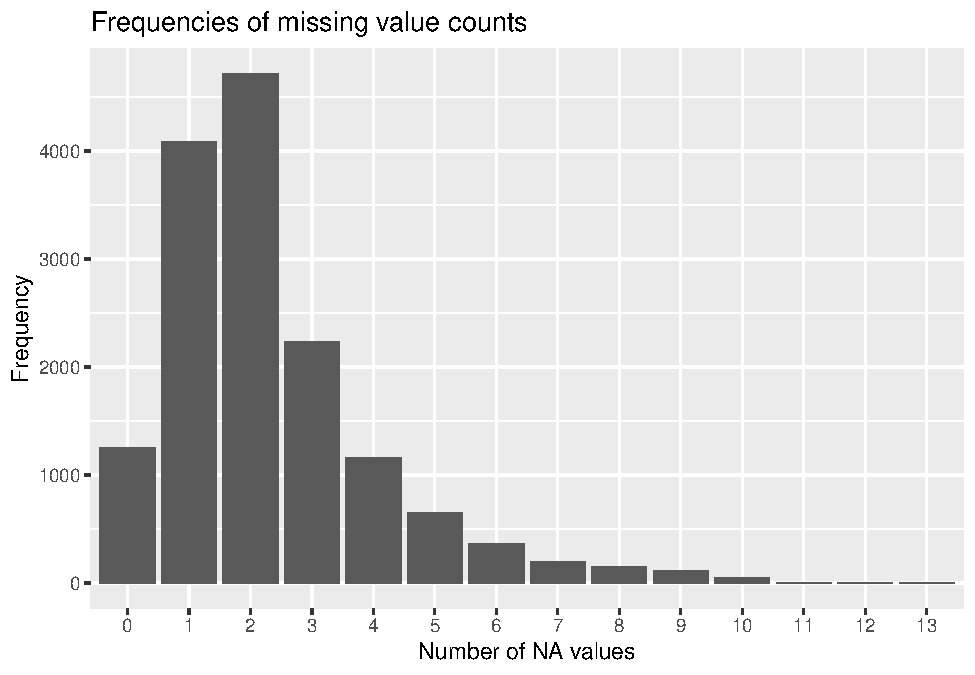
\includegraphics{hw3_files/figure-latex/unnamed-chunk-5-1.pdf}

\begin{enumerate}
\def\labelenumi{\arabic{enumi}.}
\setcounter{enumi}{2}
\tightlist
\item
  Rows tend to have fewer missing values. This can be seen in
  right-skewed distribution of the bar plot. The center of the
  distribution is around 2 missing values.
\end{enumerate}

\hypertarget{exercise-3}{%
\section{Exercise 3}\label{exercise-3}}

Make a box plot of \texttt{odometer} readings, broken down by the
\texttt{condition} of the vehicle. Remove any extreme \texttt{odometer}
values, so that it is easy to compare the boxes.

Comment briefly on the distribution of odometer readings for the various
conditions.

\emph{Hint: There are several ways to identify extreme values. One way
is to make a box plot. Another way is to find values above a certain
percentile (\texttt{quantile()}), say 99\%. Yet another way is to find
values more than 2-3 standard deviations (\texttt{sd()}) from the mean.
Each has trade-offs, but we won't focus on those in this class.}

\textbf{YOUR ANSWER GOES HERE:}

\begin{Shaded}
\begin{Highlighting}[]
\CommentTok{\# removing outliers}
\NormalTok{Q =}\StringTok{ }\KeywordTok{quantile}\NormalTok{(data}\OperatorTok{$}\NormalTok{odometer, }\DataTypeTok{probs =} \KeywordTok{c}\NormalTok{(.}\DecValTok{01}\NormalTok{, }\FloatTok{.99}\NormalTok{), }\DataTypeTok{na.rm =} \OtherTok{TRUE}\NormalTok{)}

\KeywordTok{ggplot}\NormalTok{(}\KeywordTok{subset}\NormalTok{(data, data}\OperatorTok{$}\NormalTok{odometer }\OperatorTok{\textless{}}\StringTok{ }\NormalTok{Q[}\DecValTok{2}\NormalTok{] }\OperatorTok{\&}\StringTok{ }\NormalTok{data}\OperatorTok{$}\NormalTok{odometer }\OperatorTok{\textgreater{}}\StringTok{ }\NormalTok{Q[}\DecValTok{1}\NormalTok{]),}
\KeywordTok{aes}\NormalTok{(}\DataTypeTok{x =}\NormalTok{ odometer, }\DataTypeTok{y =}\NormalTok{ condition)) }\OperatorTok{+}
\KeywordTok{geom\_boxplot}\NormalTok{()}
\end{Highlighting}
\end{Shaded}

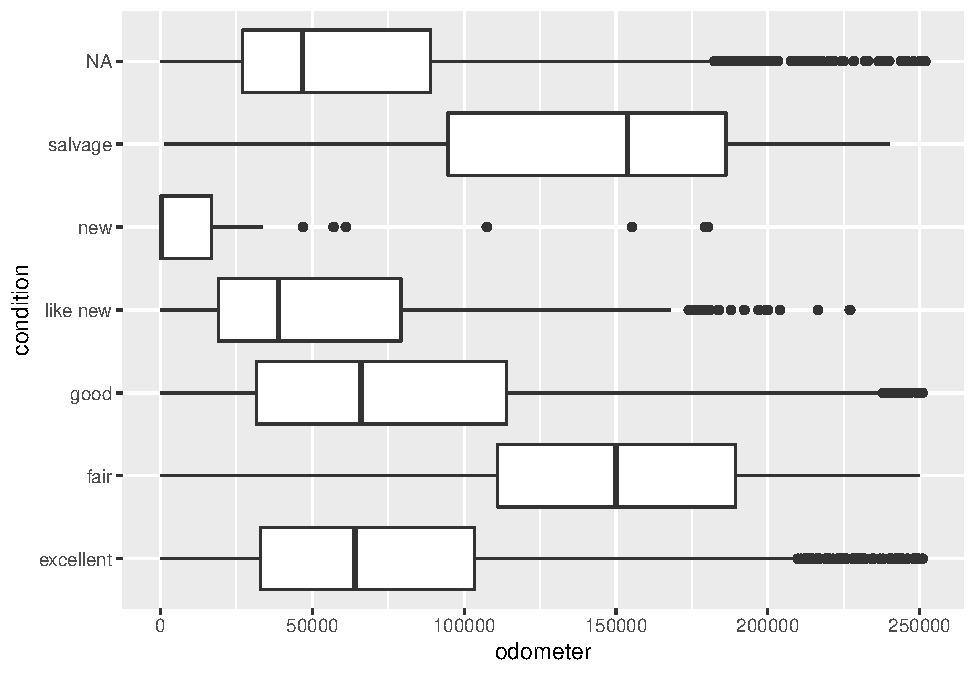
\includegraphics{hw3_files/figure-latex/unnamed-chunk-6-1.pdf} As the
condition of the car gets worse, the milage on the odometer tends to
increase. This makes sense because cars that are driven more are more
likely to be in bad condition.

\hypertarget{exercise-4}{%
\section{Exercise 4}\label{exercise-4}}

Answer each question about advertisements for vehicles \textbf{in
Berkeley}.

\emph{Hint: You might want to get started by taking a subset. Watch out
for missing values.}

\begin{enumerate}
\def\labelenumi{\arabic{enumi}.}
\item
  How many advertisements are for vehicles in Berkeley?
\item
  How many of each \texttt{type} of car are there? Which type is the
  most common?
\item
  What's the median price (ignoring missing values) of each
  \texttt{type} of car? Which type has the highest median, and which has
  the lowest?
\end{enumerate}

\textbf{YOUR ANSWER GOES HERE:}

\begin{enumerate}
\def\labelenumi{\arabic{enumi}.}
\tightlist
\item
  There are 73 advertisements for vehicles in Berkeley. This result is
  the same using either \texttt{\$place\ or\ \$city}.
\end{enumerate}

\begin{Shaded}
\begin{Highlighting}[]
\NormalTok{data\_in\_berkeley =}\StringTok{ }\KeywordTok{subset}\NormalTok{(data, data}\OperatorTok{$}\NormalTok{city }\OperatorTok{==}\StringTok{ "Berkeley"}\NormalTok{)}
\KeywordTok{nrow}\NormalTok{(data\_in\_berkeley)}
\end{Highlighting}
\end{Shaded}

\begin{verbatim}
## [1] 73
\end{verbatim}

\begin{enumerate}
\def\labelenumi{\arabic{enumi}.}
\setcounter{enumi}{1}
\tightlist
\item
  The most common type of car is \texttt{sedan} with 28 advertisements.
\end{enumerate}

\begin{Shaded}
\begin{Highlighting}[]
\KeywordTok{table}\NormalTok{(data\_in\_berkeley}\OperatorTok{$}\NormalTok{type)}
\end{Highlighting}
\end{Shaded}

\begin{verbatim}
## 
##         bus convertible       coupe   hatchback    mini-van     offroad 
##           0           2           2          11           0           0 
##       other      pickup       sedan         suv       truck         van 
##           0           2          28          12           1           3 
##       wagon 
##           2
\end{verbatim}

\begin{Shaded}
\begin{Highlighting}[]
\CommentTok{\# The mose common type of car}
\KeywordTok{head}\NormalTok{(}\KeywordTok{sort}\NormalTok{(}\KeywordTok{table}\NormalTok{(data\_in\_berkeley}\OperatorTok{$}\NormalTok{type), }\DataTypeTok{decreasing =} \OtherTok{TRUE}\NormalTok{), }\DecValTok{1}\NormalTok{)}
\end{Highlighting}
\end{Shaded}

\begin{verbatim}
## 
## sedan 
##    28
\end{verbatim}

\begin{enumerate}
\def\labelenumi{\arabic{enumi}.}
\setcounter{enumi}{2}
\tightlist
\item
  The highest median price type is \texttt{coupe} at \texttt{39300}
  while the lowest is \texttt{wagon} at \texttt{13400}.
\end{enumerate}

\begin{Shaded}
\begin{Highlighting}[]
\KeywordTok{tapply}\NormalTok{(data\_in\_berkeley}\OperatorTok{$}\NormalTok{price, data\_in\_berkeley}\OperatorTok{$}\NormalTok{type, median, }\DataTypeTok{na.rm =} \OtherTok{TRUE}\NormalTok{)}
\end{Highlighting}
\end{Shaded}

\begin{verbatim}
##         bus convertible       coupe   hatchback    mini-van     offroad 
##          NA       38150       39300       13791          NA          NA 
##       other      pickup       sedan         suv       truck         van 
##          NA       37200       15991       16993       17500       14900 
##       wagon 
##       13400
\end{verbatim}

\begin{Shaded}
\begin{Highlighting}[]
\CommentTok{\# Highest median price}
\KeywordTok{head}\NormalTok{(}\KeywordTok{sort}\NormalTok{(}\KeywordTok{tapply}\NormalTok{(data\_in\_berkeley}\OperatorTok{$}\NormalTok{price, data\_in\_berkeley}\OperatorTok{$}\NormalTok{type, median, }\DataTypeTok{na.rm =} \OtherTok{TRUE}\NormalTok{), }\DataTypeTok{decreasing =} \OtherTok{TRUE}\NormalTok{), }\DecValTok{1}\NormalTok{)}
\end{Highlighting}
\end{Shaded}

\begin{verbatim}
## coupe 
## 39300
\end{verbatim}

\begin{Shaded}
\begin{Highlighting}[]
\CommentTok{\# Lowest median price}
\KeywordTok{tail}\NormalTok{(}\KeywordTok{sort}\NormalTok{(}\KeywordTok{tapply}\NormalTok{(data\_in\_berkeley}\OperatorTok{$}\NormalTok{price, data\_in\_berkeley}\OperatorTok{$}\NormalTok{type, median, }\DataTypeTok{na.rm =} \OtherTok{TRUE}\NormalTok{), }\DataTypeTok{decreasing =} \OtherTok{TRUE}\NormalTok{), }\DecValTok{1}\NormalTok{)}
\end{Highlighting}
\end{Shaded}

\begin{verbatim}
## wagon 
## 13400
\end{verbatim}

\hypertarget{exercise-5}{%
\section{Exercise 5}\label{exercise-5}}

\begin{enumerate}
\def\labelenumi{\arabic{enumi}.}
\item
  Make a density plot of price. Use three separate lines for ads in San
  Francisco, San Jose, and Oakland (omit the other cities).

  \emph{Hint: You can use the \texttt{droplevels()} function to drop
  factor levels that aren't present.}
\item
  How do price distributions of the three cities compare?
\item
  Based on the plot, which of these cities have ads with
  extreme/anomalous prices? Isolate one of these ads. Does the extreme
  price seem accurate, or is it a mistake? Use the original title and
  text of the ad as evidence.

  \emph{Hint 1: You can print the text of an ad in human-readable form
  with the \texttt{message()} function.}

  \emph{Hint 2: You can use the \texttt{stringr} package's
  \texttt{str\_wrap()} function to wrap long strings (e.g., the ad text)
  for printing in the notebook.}

  \emph{Hint 3: The PDFLaTeX program that RMarkdown uses to knit PDFs
  only supports ASCII characters. Many of the advertisments contain
  non-ASCII characters. If you get a knit error like
  \texttt{!\ Package\ inputenc\ Error:\ Unicode\ character}, you
  probably printed an ad with non-ASCII characters.}

  \emph{To fix it, you can either comment out the line that prints the
  ad, or switch from PDFLaTeX to XeLaTeX or LuaLaTeX. See
  \url{https://bookdown.org/yihui/rmarkdown-cookbook/latex-unicode.html}
  for details about how to switch.}
\end{enumerate}

\textbf{YOUR ANSWER GOES HERE:}

\begin{enumerate}
\def\labelenumi{\arabic{enumi}.}
\tightlist
\item
\end{enumerate}

\begin{Shaded}
\begin{Highlighting}[]
\CommentTok{\# Prepare data}
\NormalTok{three\_cities\_data =}\StringTok{ }\KeywordTok{subset}\NormalTok{(data, city }\OperatorTok{==}\StringTok{ }\KeywordTok{c}\NormalTok{(}\StringTok{"San Francisco"}\NormalTok{, }\StringTok{"Oakland"}\NormalTok{, }\StringTok{"San Jose"}\NormalTok{))}
\end{Highlighting}
\end{Shaded}

\begin{verbatim}
## Warning in `==.default`(city, c("San Francisco", "Oakland", "San Jose")): longer
## object length is not a multiple of shorter object length
\end{verbatim}

\begin{verbatim}
## Warning in is.na(e1) | is.na(e2): longer object length is not a multiple of
## shorter object length
\end{verbatim}

\begin{Shaded}
\begin{Highlighting}[]
\NormalTok{three\_cities\_data}\OperatorTok{$}\NormalTok{city =}\StringTok{ }\KeywordTok{droplevels}\NormalTok{(three\_cities\_data}\OperatorTok{$}\NormalTok{city)}
\KeywordTok{levels}\NormalTok{(three\_cities\_data}\OperatorTok{$}\NormalTok{city)}
\end{Highlighting}
\end{Shaded}

\begin{verbatim}
## [1] "Oakland"       "San Francisco" "San Jose"
\end{verbatim}

\begin{Shaded}
\begin{Highlighting}[]
\KeywordTok{ggplot}\NormalTok{(three\_cities\_data, }\KeywordTok{aes}\NormalTok{(}\DataTypeTok{x =}\NormalTok{ price, }\DataTypeTok{color =}\NormalTok{ city)) }\OperatorTok{+}\StringTok{ }\KeywordTok{geom\_density}\NormalTok{() }\OperatorTok{+}
\KeywordTok{ggtitle}\NormalTok{(}\StringTok{"Desity of prices in selected cities"}\NormalTok{) }\OperatorTok{+}\StringTok{ }\KeywordTok{xlab}\NormalTok{(}\StringTok{"Price"}\NormalTok{) }\OperatorTok{+}\StringTok{ }\KeywordTok{ylab}\NormalTok{(}\StringTok{"Density"}\NormalTok{)}
\end{Highlighting}
\end{Shaded}

\begin{verbatim}
## Warning: Removed 38 rows containing non-finite values (stat_density).
\end{verbatim}

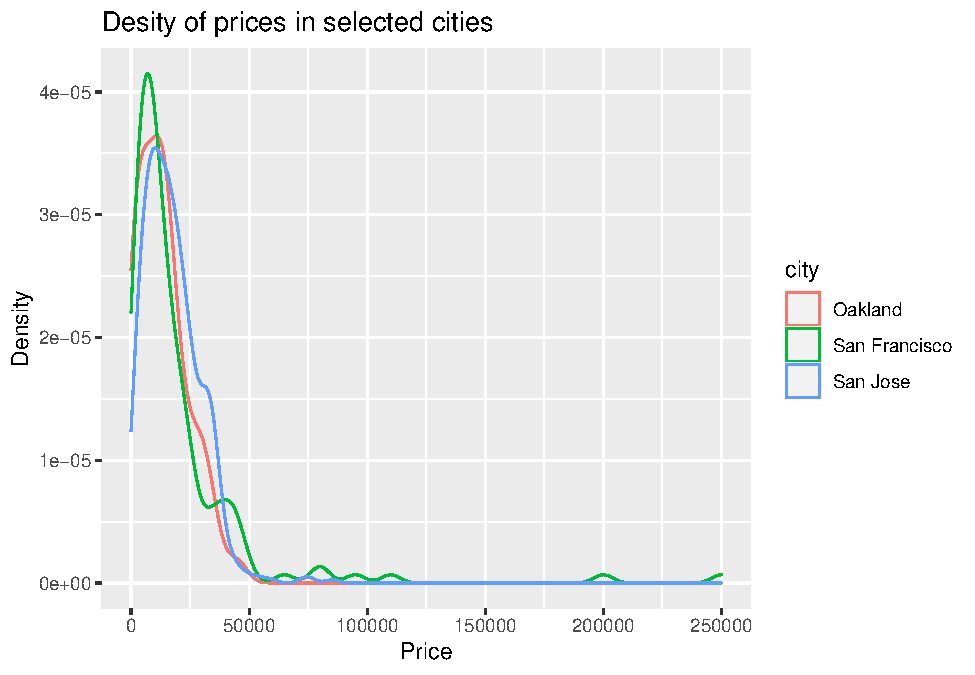
\includegraphics{hw3_files/figure-latex/unnamed-chunk-10-1.pdf}

\begin{enumerate}
\def\labelenumi{\arabic{enumi}.}
\setcounter{enumi}{1}
\item
  The price distrubutions are similar. San Francisco seems to have
  slightly higher prices.
\item
  San Francisco has some very extreme values for prices. The two most
  expensive ads are both Ferraris, so the price makes sense. The cars
  are simply very expensive.
\end{enumerate}

\begin{Shaded}
\begin{Highlighting}[]
\KeywordTok{library}\NormalTok{(stringr)}
\NormalTok{extreme\_value =}\StringTok{ }\KeywordTok{subset}\NormalTok{(three\_cities\_data, three\_cities\_data}\OperatorTok{$}\NormalTok{price }\OperatorTok{\textgreater{}}\StringTok{ }\DecValTok{240000}\NormalTok{)}
\NormalTok{extreme\_value}\OperatorTok{$}\NormalTok{title}
\end{Highlighting}
\end{Shaded}

\begin{verbatim}
## [1] "2019 Ferrari 488 GTB - 650 Score WE CARRY CONTRACTS - $249,995 (mountain view)"
\end{verbatim}

\begin{Shaded}
\begin{Highlighting}[]
\NormalTok{text \textless{}{-}}\StringTok{ }\KeywordTok{str\_c}\NormalTok{(extreme\_value}\OperatorTok{$}\NormalTok{text, }\DataTypeTok{collapse =} \StringTok{"}\CharTok{\textbackslash{}n}\StringTok{"}\NormalTok{)}
\KeywordTok{cat}\NormalTok{(}\KeywordTok{str\_wrap}\NormalTok{(text), }\StringTok{"}\CharTok{\textbackslash{}n}\StringTok{"}\NormalTok{)}
\end{Highlighting}
\end{Shaded}

\begin{verbatim}
## QR Code Link to This Post Call Adam, 18052330098 for more details! Lease for
## $1,956+ tax for 60 months. This is a commercial lease example, a consumer lease
## is available at slightly different terms. OAC for California residents only.
## To change the terms or adjust miles, go to our lease calculator for this car.
## Amazon leasing services 1100 dealers and is not a dealership. We only re-market
## a very few, very select cars at lease termination.
\end{verbatim}

\end{document}
